\documentclass[10pt,a4paper]{book}
\usepackage[utf8]{inputenc}
\usepackage[T1]{fontenc}
\usepackage{amsmath}
\usepackage{amssymb}
\usepackage{graphicx}
\usepackage{multirow}
\usepackage{tikz}
\usetikzlibrary{automata,positioning,arrows.meta}
\tikzset{
	->, % makes the edges directed
	>=stealth, % makes the arrow heads bold
	node distance=3cm, % specifies the minimum distance between two nodes. Change if necessary.
	every state/.style={thick, fill=gray!10}, % sets the properties for each ’state’ node
	initial text=$ $, % sets the text that appears on the start arrow
}
\date{}

\title{\Huge Taller automatas de pila,Gramaticas libres de contexto, Maquinas de Turing}
\author{Jojan Esteban Serna Serna\\Santiago Agredo Vallejo\\Fabian Ome Pena}
\begin{document}
	\maketitle
	\title{\huge Taller automatas de pila, Gramáticas libres de contexto y Máquinas de Turing}\\[2cm]
	1.Construya un autómata de pila que reconozca los siguientes lenguajes:\\ \\
	L1 = { SzSTz / S es una cadena de caracteres y ST su transpuesta},  L1 está definido sobre el alfabeto {a,b,z} y z no aparece en S\\
	L2 = ${ x^ny^{2n} / n>0}$\\
	L3 = El conjunto de todas las cadenas sobre el alfabeto {(,),c,d) que tienen sus paréntesis balanceados y bien anidados.\\
	\textbf{$L_1:$}
		\begin{figure*}[ht]
		%\centering
		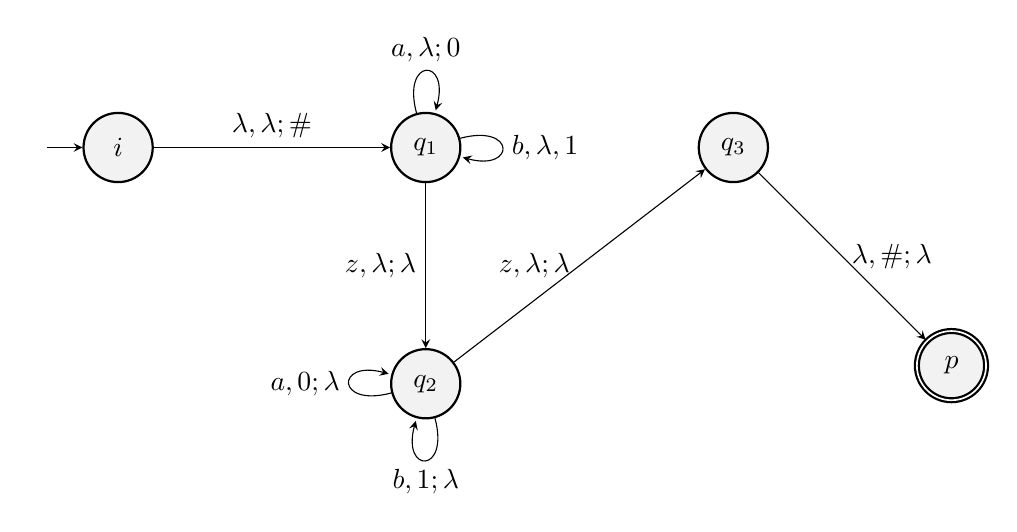
\begin{tikzpicture}
			\centering
			\node[state,initial] (i){$i$};
			\node[state,right=of i] (q1){$q_1$};
			\node[state,below of=q1] (q2){$q_2$};
			\node[state,right=of q1] (q3){$q_3$};
			\node[state,accepting,below right=of q3] (p){$p$};
			
			\draw	(i) edge[above] node{$\lambda,\lambda;\#$}  (q1)
			(q1) edge[above,loop above] node{$a,\lambda;0$} (q1)
			(q1) edge[left,loop right] node{$b,\lambda,1$} (q1)
			(q1) edge[left] node{$z,\lambda;\lambda$} (q2)
			(q2) edge[above,loop left] node{$a,0;\lambda$} (q2)
			(q2) edge[below,loop below] node{$b,1;\lambda$} (q2)
			(q2) edge[left] node{$z,\lambda;\lambda$} (q3)
			(q3) edge[right] node{$\lambda,\#;\lambda$} (p);
		\end{tikzpicture}
		\caption{NFA for $\{SzS^tz \} : L_1 = \{a,b,z\} z \notin S$}
\paragraph{$L_1:$ Definición formal}A continuación se presenta la definición formal de la maquina de pila\\[0.2cm]
\begin{alignat*}{2}
	S&= \{i, q_1, q_2, q_3, p\}\\
	\textstyle \sum&= \{a, b, z\}\\
	\Gamma&=\{1,0,\#\}\\
	T&=\{(i,\lambda,\lambda;q_1,\#),(q_1,a,\lambda;q_1,0),(q_1,b,\lambda;q_1,1),(q_1,z,\lambda;q_2,\lambda) ,(q_2,a,0;q_2,\lambda),\\&(q_2,b,1;q_2,\lambda),(q_2,z,\lambda,q_3,\lambda),(q_3,\lambda,\#;p,\lambda)    \}\\
	i&=\{i\}\\
	F&=\{\{p\}\}
\end{alignat*}
\newpage
\textbf{$L_2:$}
	\end{figure*}

	\begin{figure*}[ht]
		%\centering
		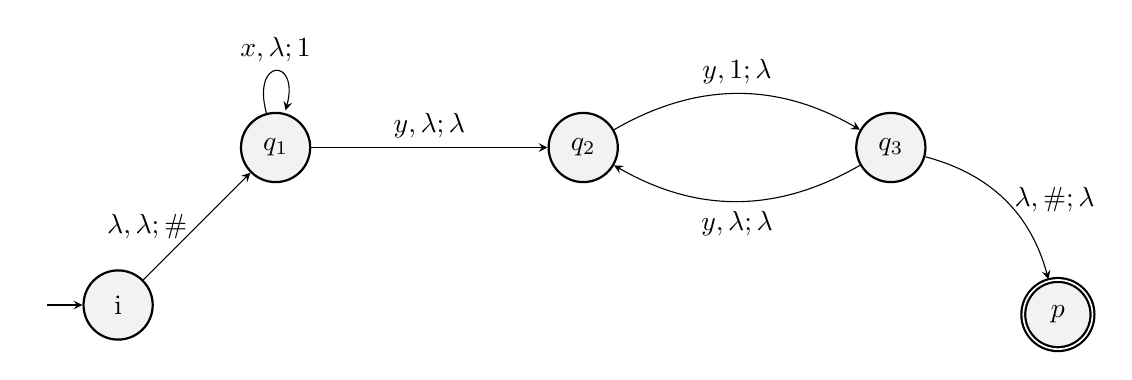
\begin{tikzpicture}
			\centering
			\node[state,initial] at (-2,-2)(i) {i};
			\node[state] (q1) {$q_1$};
			\node[state,right=of q1] (q2) {$q_2$};
			\node[state,right=of q2] (q3) {$q_3$};
			\node[state,accepting,below right of =q3] (p) {$p$};
			
			\draw (i) 	  edge[left] node{$\lambda,\lambda;\#$} (q1)
						(q1) edge[loop above] node{$x,\lambda;1$} (q1)
						(q1) edge[above] node{$y,\lambda;\lambda$} (q2)
						(q2) edge[above,bend left] node{$y,1;\lambda$} (q3)
						(q3) edge[below,bend left] node{$y,\lambda;\lambda$} (q2)
						(q3) edge[right,bend left] node{$\lambda,\#;\lambda$} (p);
						%(q1) 	edge(above) node{$y;\lambda,\lambda$}(q2)
		\end{tikzpicture}
		\caption{NFA for ${x^n y^{2n} /n>0}$}
	\end{figure*}
\newpage
\paragraph{$L_2:$ Definición formal}A continuación se presenta la definición formal de la maquina de pila\\[0.2cm]
\begin{alignat*}{2}	
	S&= \{i, q_1, q_2, q_3, p\}\\
	\textstyle \sum&= \{x,y\}\\
	\Gamma&=\{1,\#\}\\
	T&=\{(i,\lambda,\lambda,q_1,\#),(q_1,x,\lambda;q_1,1),(q_1,y,\lambda;q_2,\lambda),(q_2,y,1;q_3,\lambda),(q_3,y,\lambda;q_2,\lambda),(q_3,\lambda,\#;p,\lambda) \}\\
	i&=i\\
	F&=\{\{p\}\}
\end{alignat*}


\textbf{$L_3:$}
	\begin{figure*}[h!]
		\centering
		\begin{tikzpicture}
			\centering
			\node[state,initial] (i){$i$};
			\node[state,right=of q1] (q2) {$q_2$};
			\node[state,accepting,below right=of q2] (p) {$p$};
			
			\draw	
							(i) edge[above,bend left] node{$\lambda,\lambda;\#$} (q2)
							(q2) edge[above,loop left] node{$c/d,\lambda;\lambda$}  (q2)
							(q2) edge[below,loop below] node{$),0;\lambda$}  (q2) 
							(q2) edge[above,loop above] node{$(,\lambda;0$}  (q2)
							(q2) edge[right,bend left] node{$\lambda,\#;\lambda$} (p);
		\end{tikzpicture}
	\caption{NFA for $\{(,),c,d\}$}
	\end{figure*}
\paragraph{$L_3:$ Definición formal}A continuación se presenta la definición formal de la maquina de pila\\[0.2cm]
\begin{alignat*}{2}
	S&= \{i, q_2, p\}\\
	\textstyle \sum&= \{(, ),c,d\}\\
	\Gamma&=\{\#,0\}\\
	T&=\{(i,\lambda,\lambda;q_2,\#),(q_2,(,\lambda;q_2,0),(q_2,c/d,\lambda;q_2,\lambda),(q_2,),0;q_2,\lambda),(q_2,\lambda,\#;p,\lambda) \}\\
	i&=i\\
	F&=\{\{p\}\}
\end{alignat*}
\paragraph{}
2.Defina formalmente un autómata de pila para la gramática siguiente:\\[1cm]
$S \rightarrow A$\\
$A \rightarrow aAa$\\
$A \rightarrow bAb$\\
$A \rightarrow c$\\
\begin{figure*}[h!]
	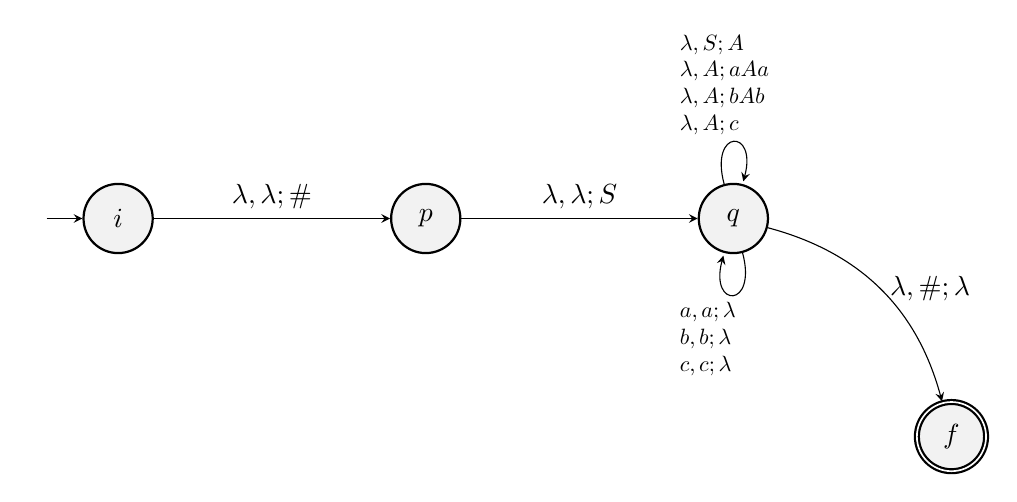
\begin{tikzpicture}
		\centering
		\node[state ,initial]  (i){$i$};
		\node[state,right=of i] (p){$p$};
		\node[state,right=of p] (q){$q$};
		\node[state,accepting,below right=of q] (f){$f$};
		
		\draw (i) edge[above] node{$\lambda,\lambda;\#$} (p)
					(p) edge[above] node{$\lambda,\lambda;S$} (q)
					(q) edge[above,loop above] node[scale=0.8,text width=1.7cm]{$\lambda,S;A$\\ $\lambda,A;aAa$\\ $\lambda,A;bAb$\\ $\lambda,A;c$} (q)
					(q) edge[below,loop below] node[scale=0.8,text width=1.7cm]{$a,a;\lambda$\\ $b,b;\lambda$ \\ $c,c;\lambda$} (q)
					(q) edge[right,bend left] node{$\lambda,\#;\lambda$} (f);
	\end{tikzpicture}
	\caption{PDA  for 2}
\end{figure*}
\paragraph{$2:$ Definición formal}A continuación se presenta la definición formal de la maquina de pila\\[0.2cm]
\begin{alignat*}{2}
	S&= \{i, p,q,f\}\\
	\textstyle \sum&= \{a,b,c\}\\
	\Gamma&=\{\#,S,A,a,b,c\}\\
	T&=\{(i,\lambda,\lambda;p,\#),(p,\lambda,\lambda;q,S),(q,\lambda,S;q,A) , (q.\lambda,A;q,aAa),(q,\lambda,A;q,bAb),(q,\lambda,A;q,c),\\&(q,a,a;q,\lambda),(q,b,b;q,\lambda),(q,c,c;q,\lambda),(q,\lambda,\#;f,\lambda)\}\\
	i&=\{i\}\\
	F&=\{\{f\}\}
\end{alignat*}
3.Defina formalmente un autómata de pila para la gramática siguiente:\\[1cm]
$S \rightarrow A$\\
$S \rightarrow C$\\
$A \rightarrow aAc$\\
$A \rightarrow aBc$\\
$B \rightarrow bBc$\\
$B \rightarrow bc$\\
$C \rightarrow aCbb$\\
$C \rightarrow abb$\\
\begin{figure*}[h!]
	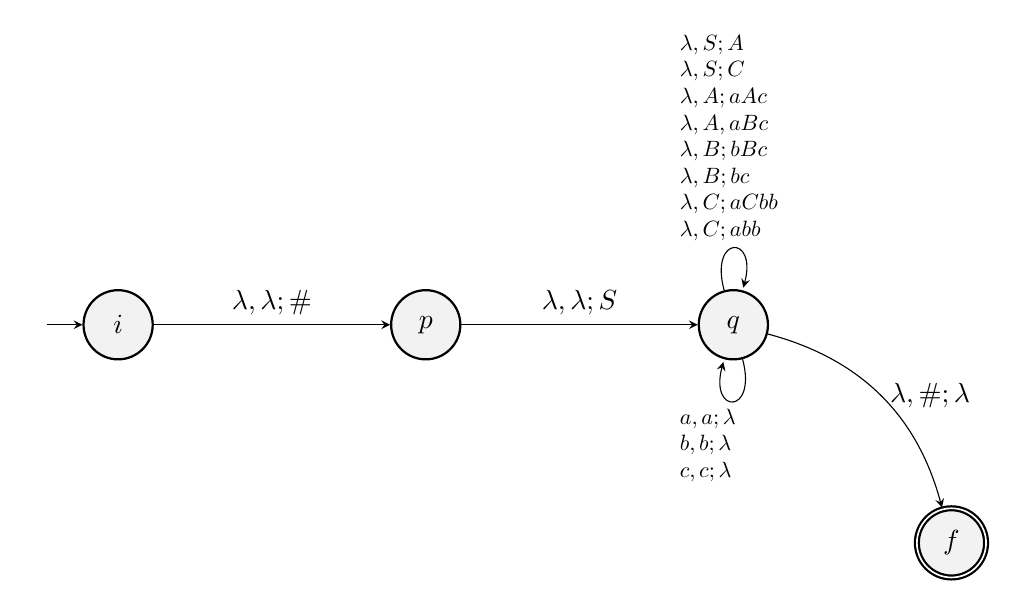
\begin{tikzpicture}
		\centering
		\node[state,initial] (i){$i$};
		\node[state,right=of i] (p){$p$};
		\node[state,right=of p] (q){$q$};
		\node[state,accepting,below right=of q] (f){$f$};
		
		\draw	(i) edge[above] node{$\lambda,\lambda;\#$} (p)
					 (p) edge[above] node{$\lambda,\lambda;S$} (q)
					 (q) edge[above, loop above] node[scale=0.8,text width=1.7cm]{$\lambda,S;A$\\$\lambda,S;C$\\$\lambda,A;aAc$\\$\lambda,A,aBc$\\$\lambda,B;bBc$\\$\lambda,B;bc$\\$\lambda,C;aCbb$\\$\lambda,C;abb$} (q)
					 (q) edge[below,loop below] node[scale=0.8,text width=1.7cm]{$a,a;\lambda$\\$b,b;\lambda$\\$c,c;\lambda$} (q)
					 (q) edge[right,bend left] node{$\lambda,\#;\lambda$} (f);
	\end{tikzpicture}
	\caption{PDA for 3}
\end{figure*}
\paragraph{$3:$ Definición formal}A continuación se presenta la definición formal de la maquina de pila\\[0.2cm]
\begin{alignat*}{2}
	S&= \{i,p,1,f\}\\
	\textstyle \sum&= \{a,b,c\}\\
	\Gamma&=\{\#,S,A,C,a,c,B,b\}\\
	T&=\{(i,\lambda,\lambda;p,\#),(p,\lambda,\lambda;q,S),(q,\lambda,S;q,A),(q,\lambda,S;q,C),(q,\lambda,A;q,aAc),(q,\lambda,A;q,aBc),(q,\lambda,B;q,bBc),\\&(q,\lambda,B;q,bc),(q,\lambda,C;q,aCbb),(q,\lambda,C;q,abb),(q,a,a;q,\lambda),(q,b,b;q,\lambda),(q,c,c;q,\lambda),(q,\lambda,\#;f,\lambda) \}\\
	i&=\{i\}\\
	F&=\{\{f\}\}
\end{alignat*}

\paragraph{}4.Diseñar una Máquina de Turing que calcule el complemento a 1 de un número binario.
(Es decir, que sustituya los 0’s por 1’s y los 1’s por 0’s).\\[1cm]
\begin{figure*}[h!]
	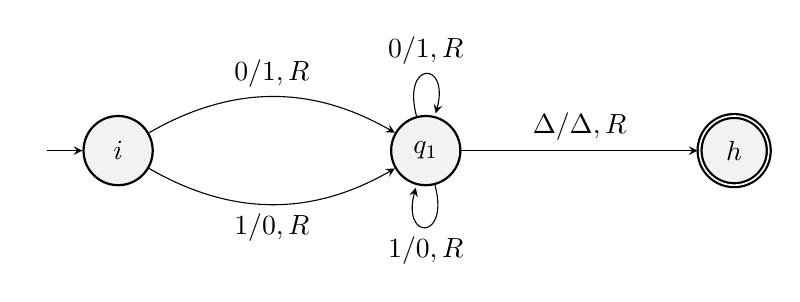
\begin{tikzpicture}
		\centering
		\node[state,initial] (i){$i$};
		\node[state,right=of i] (q1){$q_1$};
		\node[state,accepting,right=of q1] (h){$h$};
		
		\draw		(i) edge[above,bend left] node{$0/1,R$} (q1)
						  (i) edge[below,bend right] node{$1/0,R$} (q1)
						  (q1) edge[above,loop above] node{$0/1,R$}(q1)
						  (q1) edge[below,loop below] node{$1/0,R$}(q1)
						  (q1) edge[above] node{$\Delta/\Delta,R$} (h);
	\end{tikzpicture}
\end{figure*}

\paragraph{$4:$ Definición formal}A continuación se presenta la definición formal de la maquina de turing\\[0.2cm]
\begin{alignat*}{2}
	S&= \{i,q_1,h\}\\
	\textstyle \sum&= \{0,1\}\\
	\Gamma&=\{0,1\}\\
	\delta&=\{[(i,0)=(q_1,1R)],[(i,1)=(q_1,0R)],[(q_1,0)=(q_1,1R)],[(q_1,1)=(q_1,0R)],\\&[(q_1,\Delta)=(h,\Delta R)]\}\\
	i&=\{i\}\\
	h&=\{\{h\}\}
\end{alignat*}
\newpage

\paragraph{}5.Diseñar una Máquina de Turing que calcule la paridad de un número binario. Es decir, si el número de 1’s de la cadena es par, se añade un 0 al final, y si es impar, se añade un1\\[1cm]
\begin{figure*}[ht!]
	\centering
	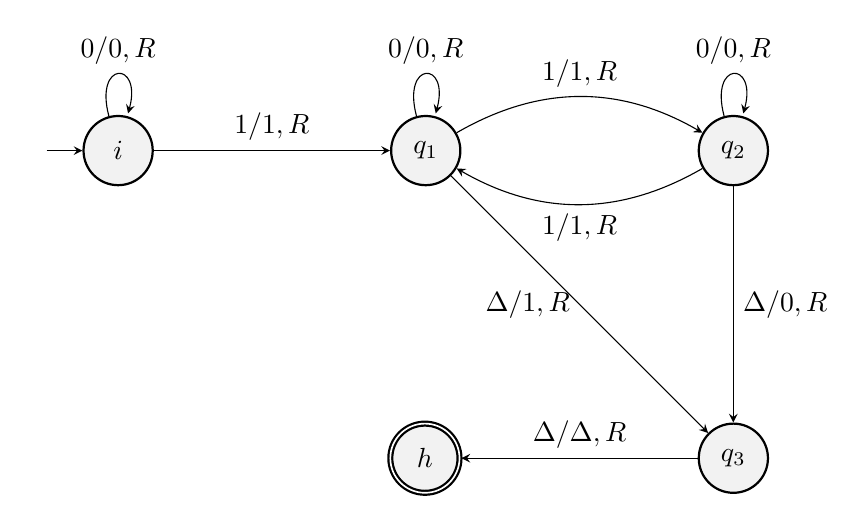
\begin{tikzpicture}
		\node[state,initial] (i){$i$};
		\node[state,right=of i] (q1){$q_1$};
		\node[state,right=of q1] (q2){$q_2$};
		\node[state,below =of q2] (q3){$q_3$};
		\node[state,accepting,left=of q3] (h){$h$};
		
		\draw	(i) edge[above,loop above] node{$0/0,R$} (i)
					  (i) edge[above] node{$1/1,R$} (q1)
					  (q1) edge[above,loop above] node{$0/0,R$} (q1)
					  (q1) edge[above,bend left] node{$1/1,R$} (q2)
					  (q2) edge[above,loop above] node{$0/0,R$} (q2)
					  (q2) edge[below,bend left] node{$1/1,R$} (q1)
					  (q2) edge[right] node{$\Delta/0,R$} (q3)
					  (q1) edge[left] node{$\Delta/1,R$} (q3)
					  (q3) edge[above] node{$\Delta/\Delta,R$} (h);
		
	\end{tikzpicture}
\end{figure*}
\paragraph{$5:$ Definición formal}A continuación se presenta la definición formal de la maquina de turing\\[0.2cm]
\begin{alignat*}{2}
	S&= \{i, q_1, q_2, q_3, h\}\\
	\textstyle \sum&= \{0,1\}\\
	\Gamma&=\{0,1\}\\
	\delta&=\{[(i,0)=(i,0R)],[(i,1)=(q_1,1R)] ,[(q_1,0)=(q_1,0R)],[(q_1,1)=(q_2,1R)],[(q_2,0)=(q_2,0R)],\\&[(q_2,1)=(q_1,1R)],[(q_1,\Delta)=(q_3,1R)],[(q_2,\Delta)=(q_3,0R)],[(q_3,\Delta)=(h,\Delta R)] \}\\
	i&=\{i\}\\
	h&=\{\{h\}\}
\end{alignat*}
\newpage
\paragraph{}6.Diseñar una Máquina de Turing que sea un contador unario de caracteres del lenguaje con alfabeto $\sum = {a,b,c}$. Es decir, se deben devolver tantos 1’s como caracteres haya en la palabra de entrada. Es decir en la cinta deben quedar tantos 1 como caracteres se encuentren en la cinta.\\[1cm]
\begin{figure*}[ht!]
	\centering
	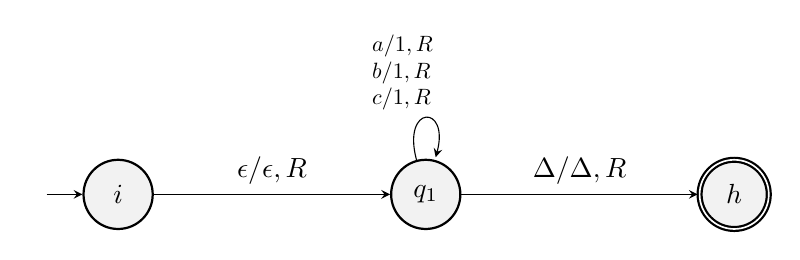
\begin{tikzpicture}
		\node[state,initial] (i){$i$};
		\node[state,right=of i] (q1){$q_1$};
		\node[state,accepting,right=of q1] (h){$h$};
		
		\draw
		(i) edge[above] node{$\epsilon/\epsilon,R$} (q1)
		(q1) edge[above,loop above] node[scale=0.8,text width=1.7cm]{$a/1,R$\\$b/1,R$\\$c/1,R$\\} (q1)

		(q1) edge[above] node{$\Delta/\Delta,R$} (h);
		
	\end{tikzpicture}
\end{figure*}
\paragraph{$6:$ Definición formal}A continuación se presenta la definición formal de la maquina de turing\\[0.2cm]
\begin{alignat*}{2}
	S&= \{i, q_1,h\}\\
	\textstyle \sum&= \{a,b,c\}\\
	\Gamma&=\{1\}\\
	\delta&=\{[(i,\epsilon), (q_1,\epsilon,R)], [(q1,a), (q1,1,R)], [(q1,b), (q1,1,R)], [(q1,c), (q1,1,R)],\\& [(q1,\Delta), (h,\Delta,R)]\}\\
	i&=\{i\}\\
	h&=\{\{h\}\}
\end{alignat*}
\newpage
\paragraph{}7. Diseñar una Máquina de Turing que sea un contador unario de caracteres del lenguaje con alfabeto $\sum = {a,b,c}$. Es decir, se deben devolver tantos 1’s como caracteres haya en la palabra de entrada. Considerar la codificación unaria del 0 igual que en el ejercicio 2.\\[1cm]
\begin{figure*}[ht!]
	\centering
	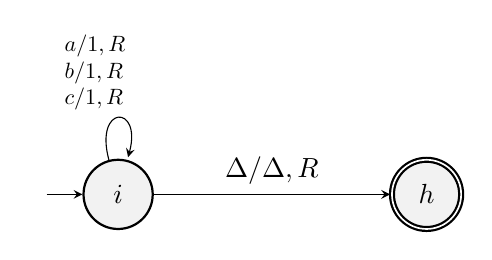
\begin{tikzpicture}
		\node[state,initial] (i){$i$};
		\node[state,accepting,right=of i] (h){$h$};
		
		\draw
		(i) edge[above,loop above] node[scale=0.8,text width=1.7cm]{$a/1,R$\\$b/1,R$\\$c/1,R$\\} (q1)
		(i) edge[above] node{$\Delta/\Delta,R$} (h);
	\end{tikzpicture}
\end{figure*}

\paragraph{$7:$ Definición formal}A continuación se presenta la definición formal de la maquina de turing\\[0.2cm]
\begin{alignat*}{2}
	S&= \{i, h\}\\
	\textstyle \sum&= \{a,b,c\}\\
	\Gamma&=\{1\}\\
	\delta&=\{[(i,a), (i,1,R)], [(i,b), (i,1,R)], [(i,c), (i,1,R)], [(i,\Delta), (h,\Delta,R)]\}\\
	i&=\{i\}\\
	h&=\{\{h\}\}
\end{alignat*}
\end{document}